%%%%%%%%%%%%%%%%%%%%%%%%%%%%%%%%%%%%%%%%%%%%%%%%%%%%%%%%%%%%%%%%%%% 
%                                                                 %
%                           CHAPTER 4                             %
%                                                                 %
%%%%%%%%%%%%%%%%%%%%%%%%%%%%%%%%%%%%%%%%%%%%%%%%%%%%%%%%%%%%%%%%%%% 
 
\chapter{Dramatic inner-core tropopause variability during the rapid intensification of {Hurricane Patricia} (2015)}
\resetfootnote %this command starts footnote numbering with 1 again.

%---------------------------------------------------------------------------------------%
\section{Introduction}
%---------------------------------------------------------------------------------------%

Hurricane Patricia became the strongest recorded hurricane in the Western Hemisphere after undergoing remarkably rapid intensification (RI) between 21 and 23 October 2015 (\citeauthor{Kimberlainetal2016} \citeyear{Kimberlainetal2016}; \citeauthor{Rogersetal2017} \citeyear{Rogersetal2017}).

Throughout this RI period, a NASA WB-57 aircraft flying in the stratosphere deployed 244 dropsondes as part of the Office of Naval Research Tropical Cyclone Intensity (TCI) Experiment \cite{DoyleTCI}.
These dropsondes revealed dramatic changes in upper-level static stability and cold-point tropopause structure throughout Patricia’s RI.

%---------------------------------------------------------------------------------------%
\section{Data and methods}
%---------------------------------------------------------------------------------------%
The High-Definition Sounding System (HDSS) provides a new capability to deploy and track up to 40 expendable digital dropsondes (XDDs) simultaneously.
This capability permits the rapid deployment of many dropsondes, providing cross sections of pressure, temperature, humidity, and wind velocity with unprecedented horizontal resolution.
\cite{Blacketal2017} report that XDDs are able to resolve atmospheric features in a manner comparable to RD-94 dropsondes \cite{HockFranklin1999}, operational rawinsondes, and aircraft spiral profiles.
The XDDs exhibited a warm bias of 18C and a dry bias of 5\% relative to RD-94 dropsondes.
XDD thermodynamic measurements, like those of other in situ sounding instruments, were noisy and unreliable when the sensors became wet.
An intensive quality control procedure \cite{BellTCI} removed unrealistic temperature and humidity observations that likely reflected sensor wetting, as well as relative humidity recorded at temperatures below -40\textdegree{}C, where humidity measurements were inaccurate because of slow sensor response time.
A more complete description of HDSS’s specifications and error characteristics can be found in \cite{Blacketal2017} and \cite{DoyleTCI}, and a comprehensive description of tihe quality control procedure in \cite{BellTCI}.

Flying near 18.5-km altitude aboard the NASA WB-57 aircraft, HDSS deployed dropsondes with horizontal spacing as small as 4 km in the inner core of TC Patricia.
This dataset builds upon that of the high-altitude dropsonde observations collected by the NASA Hurricane and Severe Storm Sentinel (HS3) investigation \cite{Braunetal2016}.
Although many dropsondes were deployed during each HS3 flight, the typical spacing of 50–200 km was not sufficient to resolve the inner core of a hurricane. In contrast, the average dropsonde spacing for the four complete transects that TCI conducted through the center of TC Patricia ranged from 4.4 to 8.0 km. 
These four flight legs, shown in Fig.~\ref{fig:patricia_ir}, will be used to analyze the upper-tropospheric and lower-stratospheric evolution of TC Patricia during its RI.

The infrared (IR) brightness temperature images plotted in Fig.~\ref{fig:patricia_ir} were parallax-corrected using Man
computer Interactive Data Access System (McIDAS-X; \citeauthor{Lazzaraetal1999} \citeyear{Lazzaraetal1999}), assuming a cloud-top height of 15 km.
For each transect, the parallax adjustment was determined at every dropsonde position and the IR image was shifted by the average of these adjustment factors.
This effectively shifted the IR image 9 km to the southeast on 21 October (when the satellite image came from GOES-13) and 13 km to the southwest on 22 and 23 October (when the satellite image came from GOES-15).
This parallax adjustment was performed only to show more realistic dropsonde deployment locations relative to the IR brightness temperatures in Fig.~\ref{fig:patricia_ir}; it did not impact any calculated field.

Each sounding in the quality-controlled TCI dropsonde dataset \citep{BellTCI} was interpolated to a 100-m vertical grid following \cite{MolinariVollaro2010}.
The static stability was analyzed using the squared Brunt–V{\"a}is{\"a}l{\"a} frequency:
   \begin{equation} \label{eq:n2dry}
   N^2 = \frac{g}{\theta}\frac{\Delta \theta}{\Delta z},
   \end{equation}
where $\Delta z$ is 200 m.
The vertical temperature gradient, $\Delta T/\Delta z$, also was computed across 200-m layers using centered finite differences.

The evolution of $\theta$ anomalies will be used to aid the diagnosis of static stability changes.
Although many previous papers have used the \cite{Jordan1958} or \cite{Dunion2011} mean soundings to compute temperature anomalies, neither of these soundings are representative of the environment in which Patricia was embedded.
For this reason, a mean state was defined using an average of 74 rawinsonde observations obtained from the University of Wyoming upper-air sounding archive \citep{Wyoming2016}.
These observations constituted all rawinsondes released from Manzanillo and Acapulco, Mexico, during October 2015. Each sounding was visually inspected for errors and three soundings from Manzanillo were removed from the average: 0000 UTC 6 October, 1200 UTC 11 October, and 1200 UTC 21 October.
These soundings exhibited unrealistically large upper-tropospheric temperature departures relative to the previous and subsequent soundings.
Their removal did not significantly alter the mean sounding: the maximum difference in the average temperatures computed with and without those soundings was 0.47\textdegree{}C. 
A total of 58 of the 74 rawinsondes reported data up to at least the 19-km level, facilitating the computation of $\theta$ anomalies well into the lower stratosphere.

For each cross section, the storm center location was determined using a wind center track produced by NOAA’s Hurricane Research Division (available online at \url{http://www.aoml.noaa.gov/hrd/Storm_pages/patricia2015/patricia.trak}).
The WB-57 dropsonde deployment location nearest this storm center estimate in space and time was used to define the center (radius = 0) for each cross section.
The distance between the nearest dropsonde and the storm track never exceeded 8.1 km (Table~\ref{table1}).
Storm-relative radial and tangential velocities were computed using the speed and direction of motion along this track.

%---------------------------------------------------------------------------------------%
\section{Results}
%---------------------------------------------------------------------------------------%

The center-crossing transects on 21, 22, and 23 October 2015 are shown in Figs. \ref{fig:patricia_ir}a-d, overlaid on infrared brightness temperature images from GOES.
Stars indicate dropsonde deployment locations and range rings are plotted every 20 km.
Brightness temperatures colder than -80\textdegree{}C extended over a broad region of Patricia’s circulation on 21 October (Fig. \ref{fig:patricia_ir}a, pink shading).
Convection was asymmetric about the storm center, with the coldest brightness temperatures (colder than -86\textdegree{}C) confined to a region 60–80 km west of Patricia’s center of circulation.
By 22 October, Patricia had rapidly intensified to a category 3 hurricane (Fig. \ref{fig:vmax}), with an eye beginning to clear in the infrared (Figs. \ref{patricia_ir}b,c).
This rapid intensification continued over the next 18 h until the storm’s maximum sustained wind speed reached its peak
of 185 kt (1 kt = 0.5144 m s\textsuperscript{-1}) at 1200 UTC 23 October (Fig. \ref{fig:vmax}; \citeauthor{Kimberlainetal2016} \citeyear{Kimberlainetal2016}).
TCI conducted its final flight into Patricia shortly thereafter, crossing over the eye around 2000 UTC (Fig. \ref{fig:patricia_ir}d) as the storm begain to weaken.



%---------------------------------------------------------------------------------------%
%FIGURES AND TABLES
%---------------------------------------------------------------------------------------%

%Table 1%

\begin{table}
  \scriptsize
 \begin{center}
   \begin{tabular}{ c c c c }
   Time and Date & Storm center from HRD track & Location of nearest WB-57 dropsonde deployment & Separation distance\\
   \hline
   \hline
   1957:00 UTC 21 Oct & 13.056\textdegree{}N, 99.244\textdegree{}W & 12.983\textdegree{}N, 99.235\textdegree{}W & 8.1 km\\
   1823:15 UTC 22 Oct & 15.123\textdegree{}N, 104.149\textdegree{}W & 15.101\textdegree{}N, 104.142\textdegree{}W & 2.5 km\\
   1906:00 UTC 22 Oct & 15.238\textdegree{}N, 104.247\textdegree{}W & 15.204\textdegree{}N, 104.237\textdegree{}W & 3.9 km\\
   2001:30 UTC 23 Oct & 18.617\textdegree{}N, 105.199\textdegree{}W & 18.590\textdegree{}N, 105.207\textdegree{}W & 3.1 km\\
   \hline
   \end{tabular}
 \end{center}
 \caption{Storm center positions from NOAA’s Hurricane Research Division (HRD) zero wind center track for Hurricane Patricia, the nearest WB-57 dropsonde deployment location, and the distance (km) between the two points.}
 \label{table1}
\end{table}

%FIGURE 1%
\begin{figure*}[ht]
\centerline{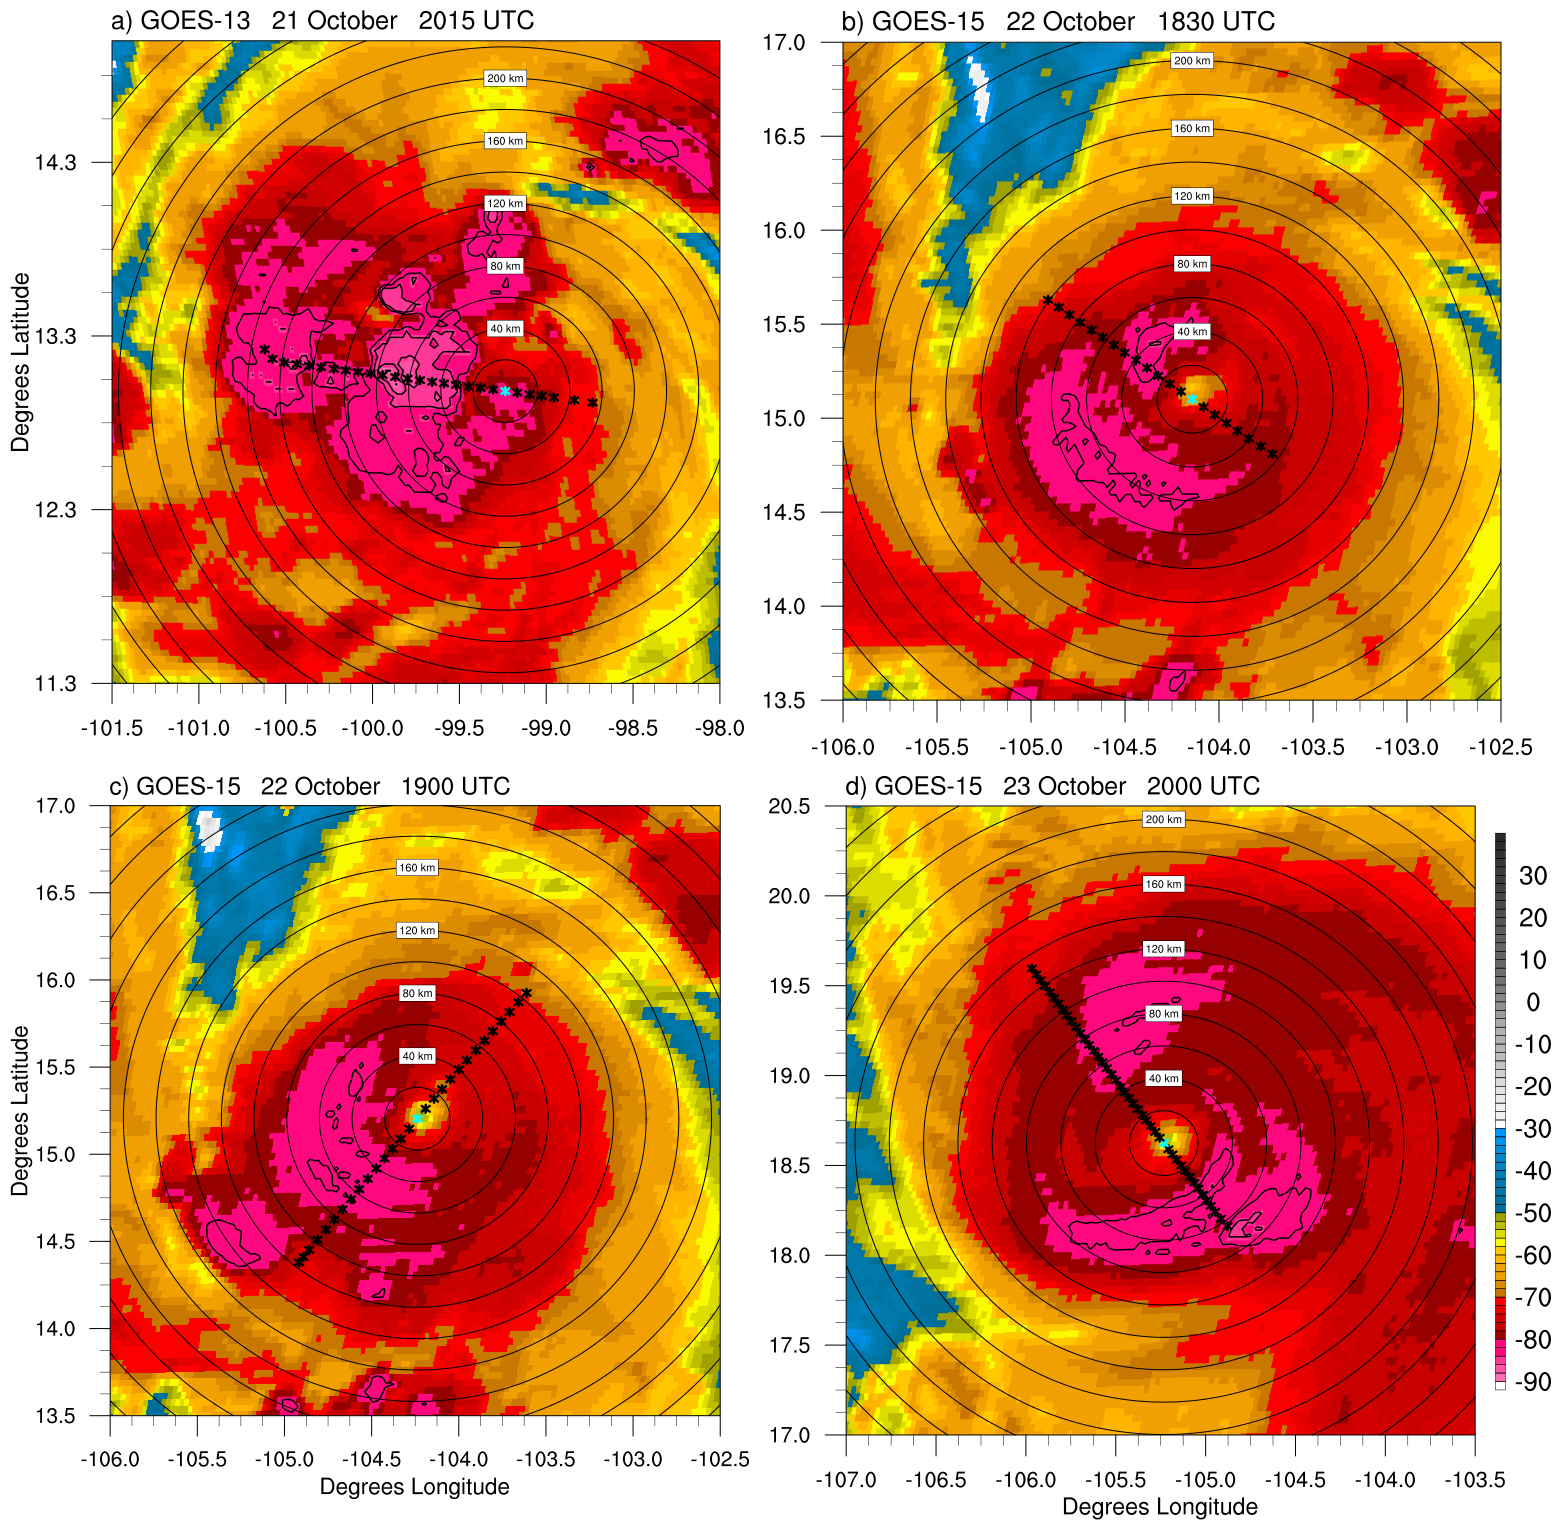
\includegraphics[width=39pc]{figures/fig01_patricia_ir.png}}
\caption{Infrared brightness temperature (\textdegree{}C) images of Tropical Storm Patricia at (a) 2015 UTC 21 Oct, and Hurricane Patricia at (b) 1830 UTC 22 Oct, (c) 1900 UTC 22 Oct, and (d) 2000 UTC 23 Oct 2015. Stars represent dropsonde deployment locations, with cyan stars marking the center location used for each cross section. Black contours delineate the coldest brightness temperatures, with a contour interval of 2\textdegree{}C starting at -82\textdegree{}C. The mean dropsonde spacing is (a) 7.9, (b) 7.8, (c) 8.0, and (d) 4.4 km for the four flight legs. Range rings are plotted every 20 km.}
\label{fig:patricia_ir}
\end{figure*}

%FIGURE 2%
\begin{figure*}[ht]
\centerline{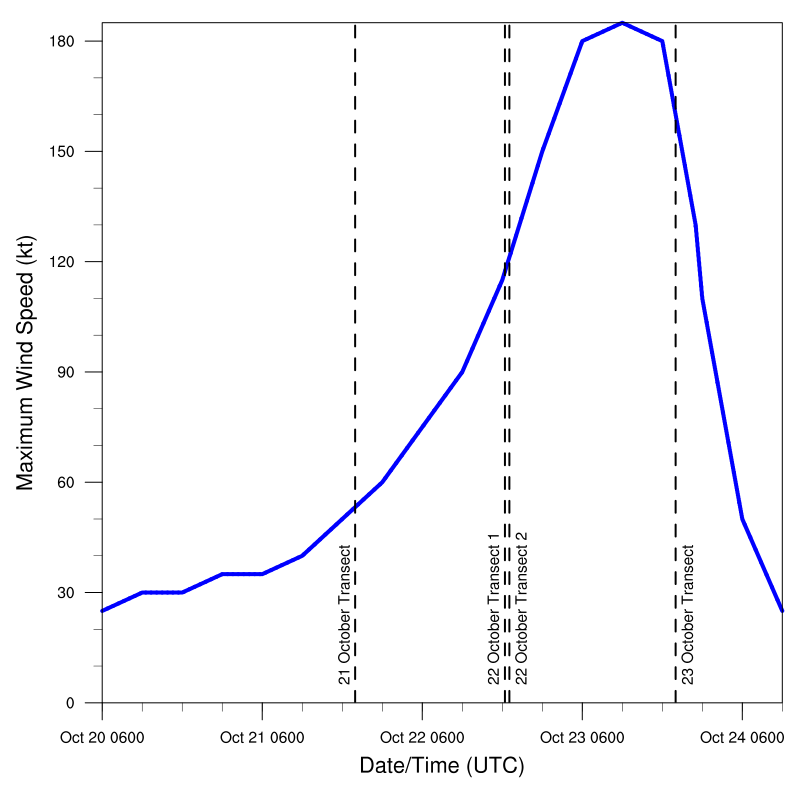
\includegraphics[width=39pc]{figures/fig02_patricia-intensity.png}}
\caption{The maximum wind speed (kt; blue line) throughout Patricia’s lifetime recorded in the National Hurricane Center best track \citep{Kimberlainetal2016}. Vertical lines indicate the times at which the WB-57 passed over the storm center during the four transects shown in Fig. \ref{fig:patricia_ir}.}
\label{fig:vmax}
\end{figure*}

%FIGURE 3%
\begin{figure*}[ht]
\centerline{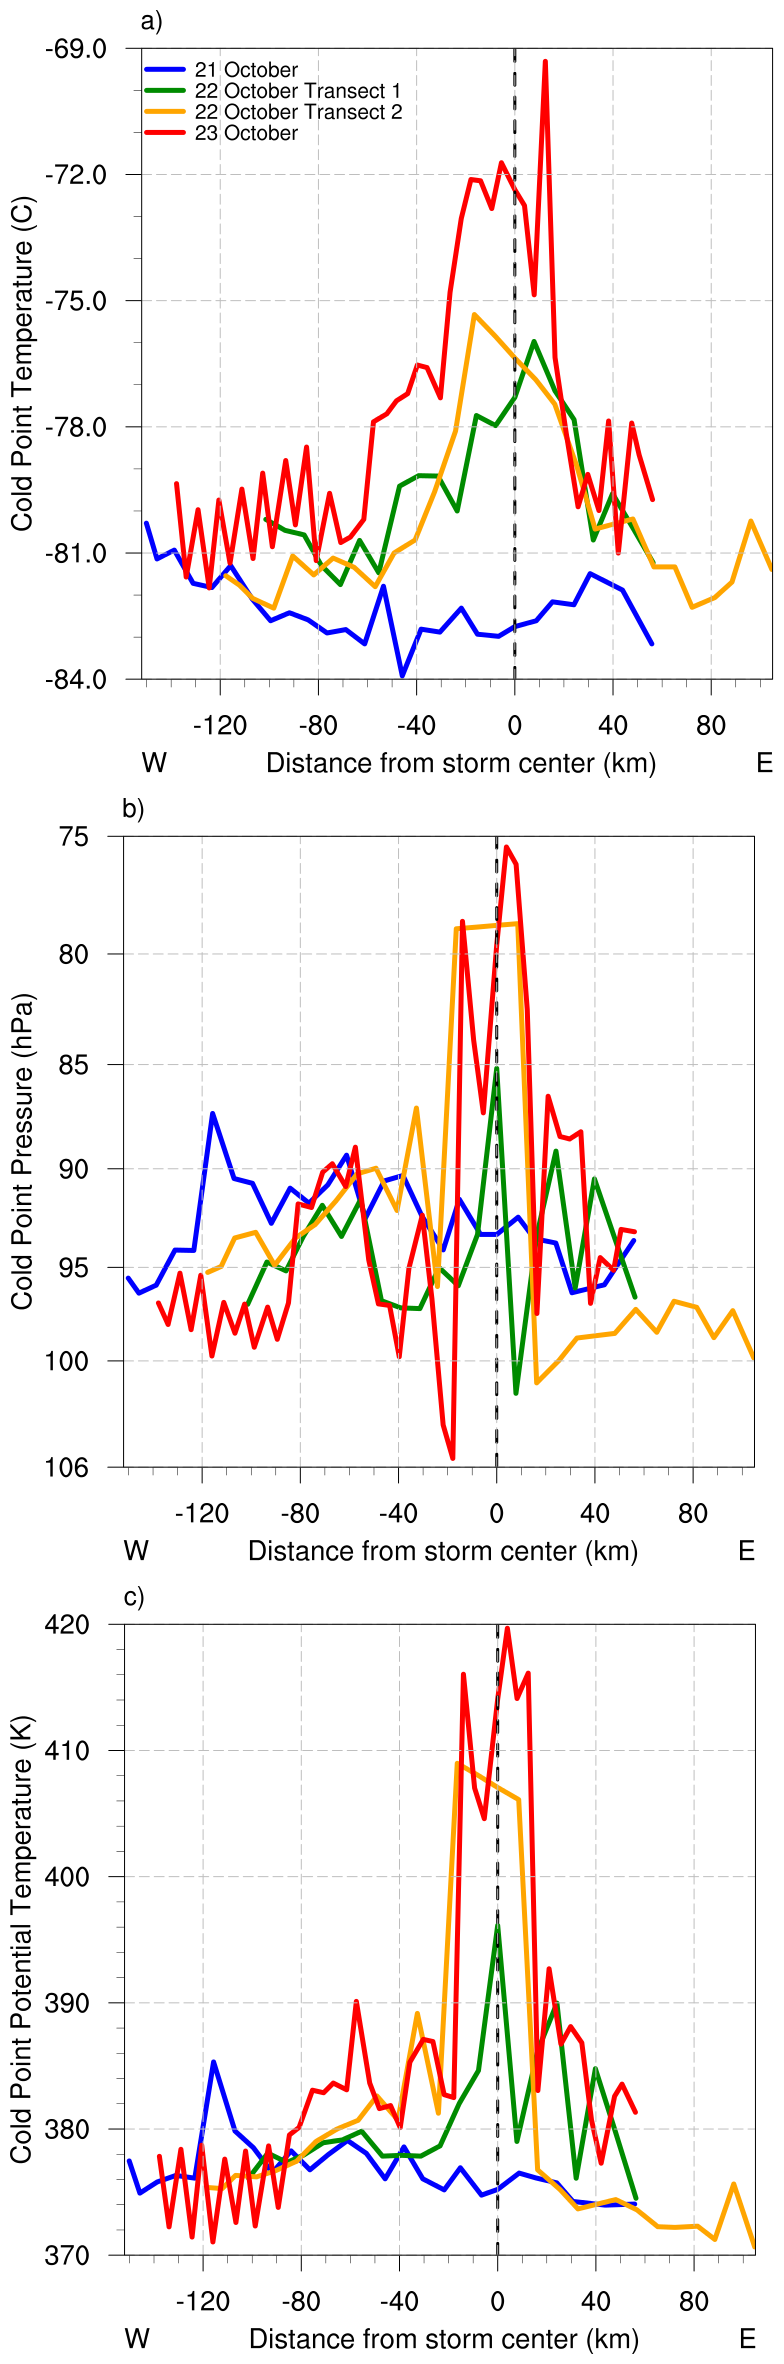
\includegraphics[width=16pc]{figures/fig03_cp_temp+theta+pres.png}}
\caption{(a) Temperature (\textdegree{}C), (b) pressure (hPa), and (c) potential temperature (K) at the cold-point tropopause for flights through the center of Tropical Storm Patricia at 1957 UTC 21 Oct (blue), and Hurricane Patricia at 1823 UTC 22 Oct (green), 1906} UTC 22 Oct (orange), and 2001 UTC 23 Oct (red) 2015. The vertical dashed lines represent the storm center. Compass directions are indicated by letters at each end of the cross section.
\label{fig:trop}
\end{figure*}

%FIGURE 4%
\begin{figure*}[ht]
\centerline{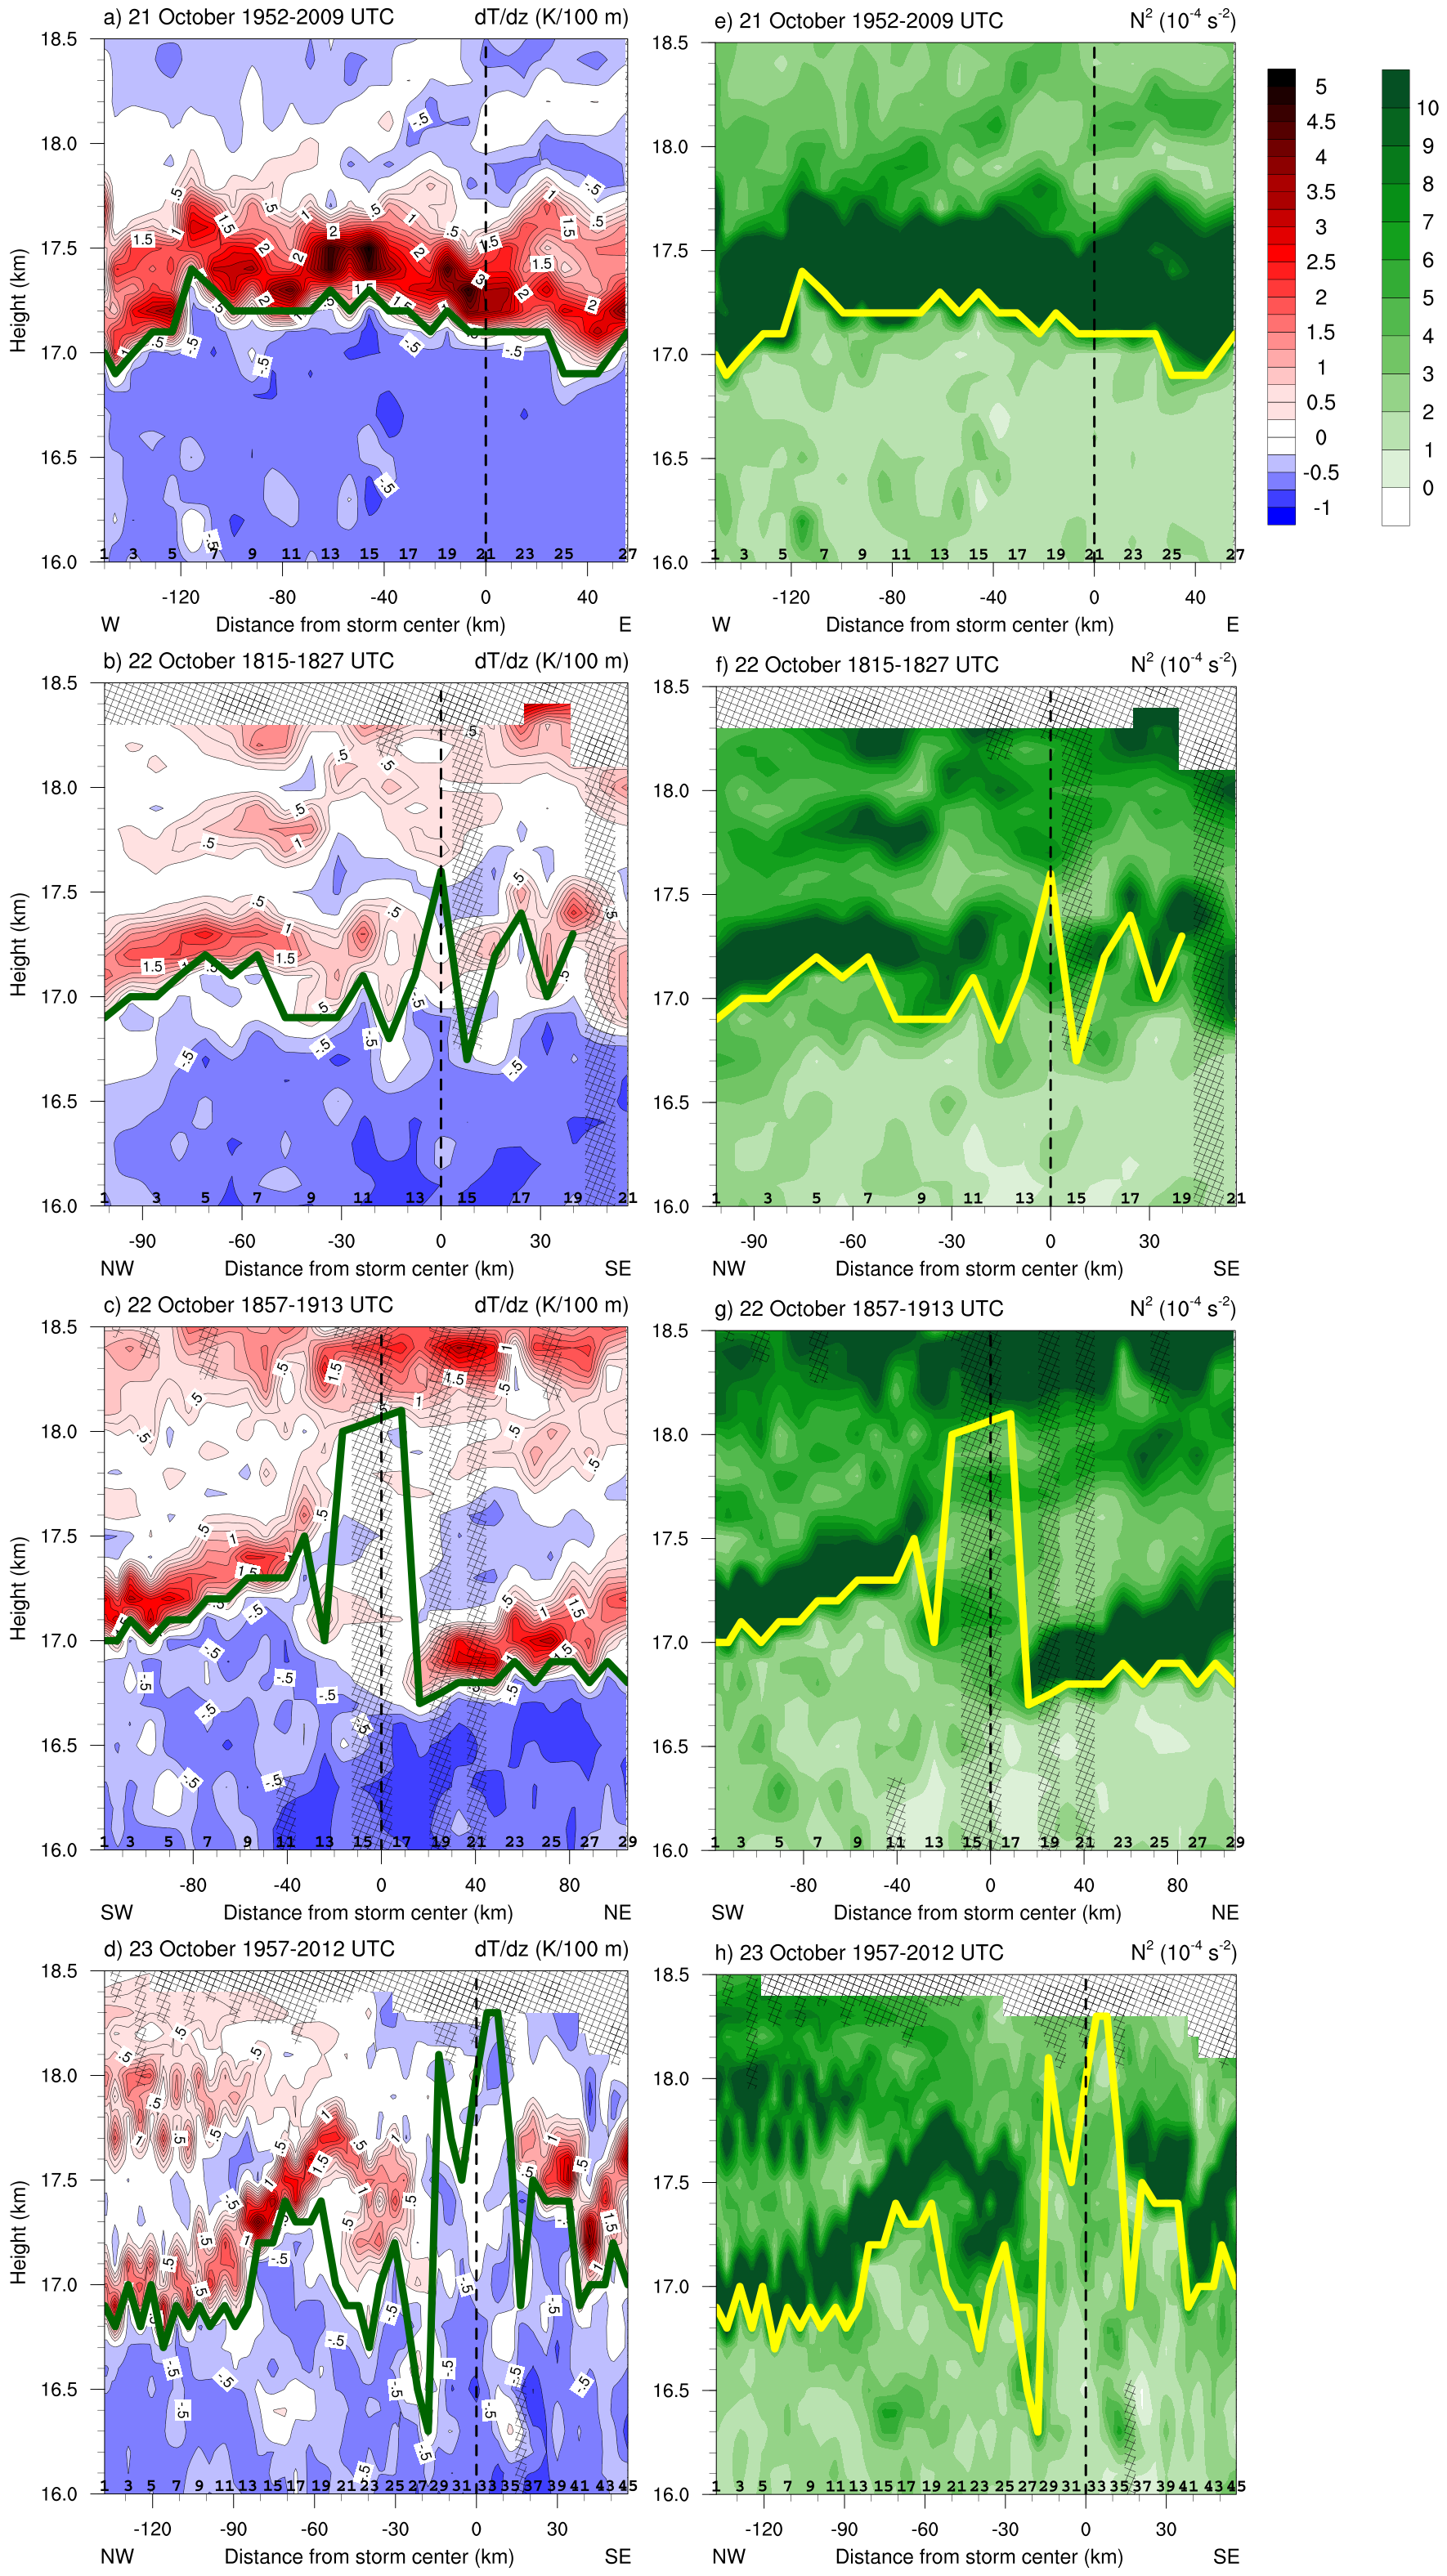
\includegraphics[width=24pc]{figures/fig04_dtdz+stab.png}}
\caption{(left) Vertical cross sections of $\Delta T/\Delta z$ [K (100 m)\textsuperscript{-1}; filled contours] and the cold-point tropopause height (green lines) along the transects shown in Fig. 1 on (a) 21; (b),(c) 22; and (d) 23 Oct 2015. Numbers along the bottom of each cross section represent the dropsonde deployment locations shown in Fig. 1 (only odd-numbered dropsondes are labeled here), with number 1 corresponding to the westernmost dropsonde. Compass directions are indicated by letters at each end of the cross sections. Dashed vertical lines mark the storm center and hatching indicates regions of missing values, where linear interpolation is performed in the radial direction. (right) Vertical cross sections of Brunt–Väisälä frequency squared (10\textsuperscript{-4} s\textsuperscript{-2}; filled contours) and cold-point tropopause height (yellow lines) on (e) 21; (f),(g) 22; and (h) 23 Oct 2015.}
\label{fig:stab}
\end{figure*}

%FIGURE 5%
\begin{figure*}[ht]
\centerline{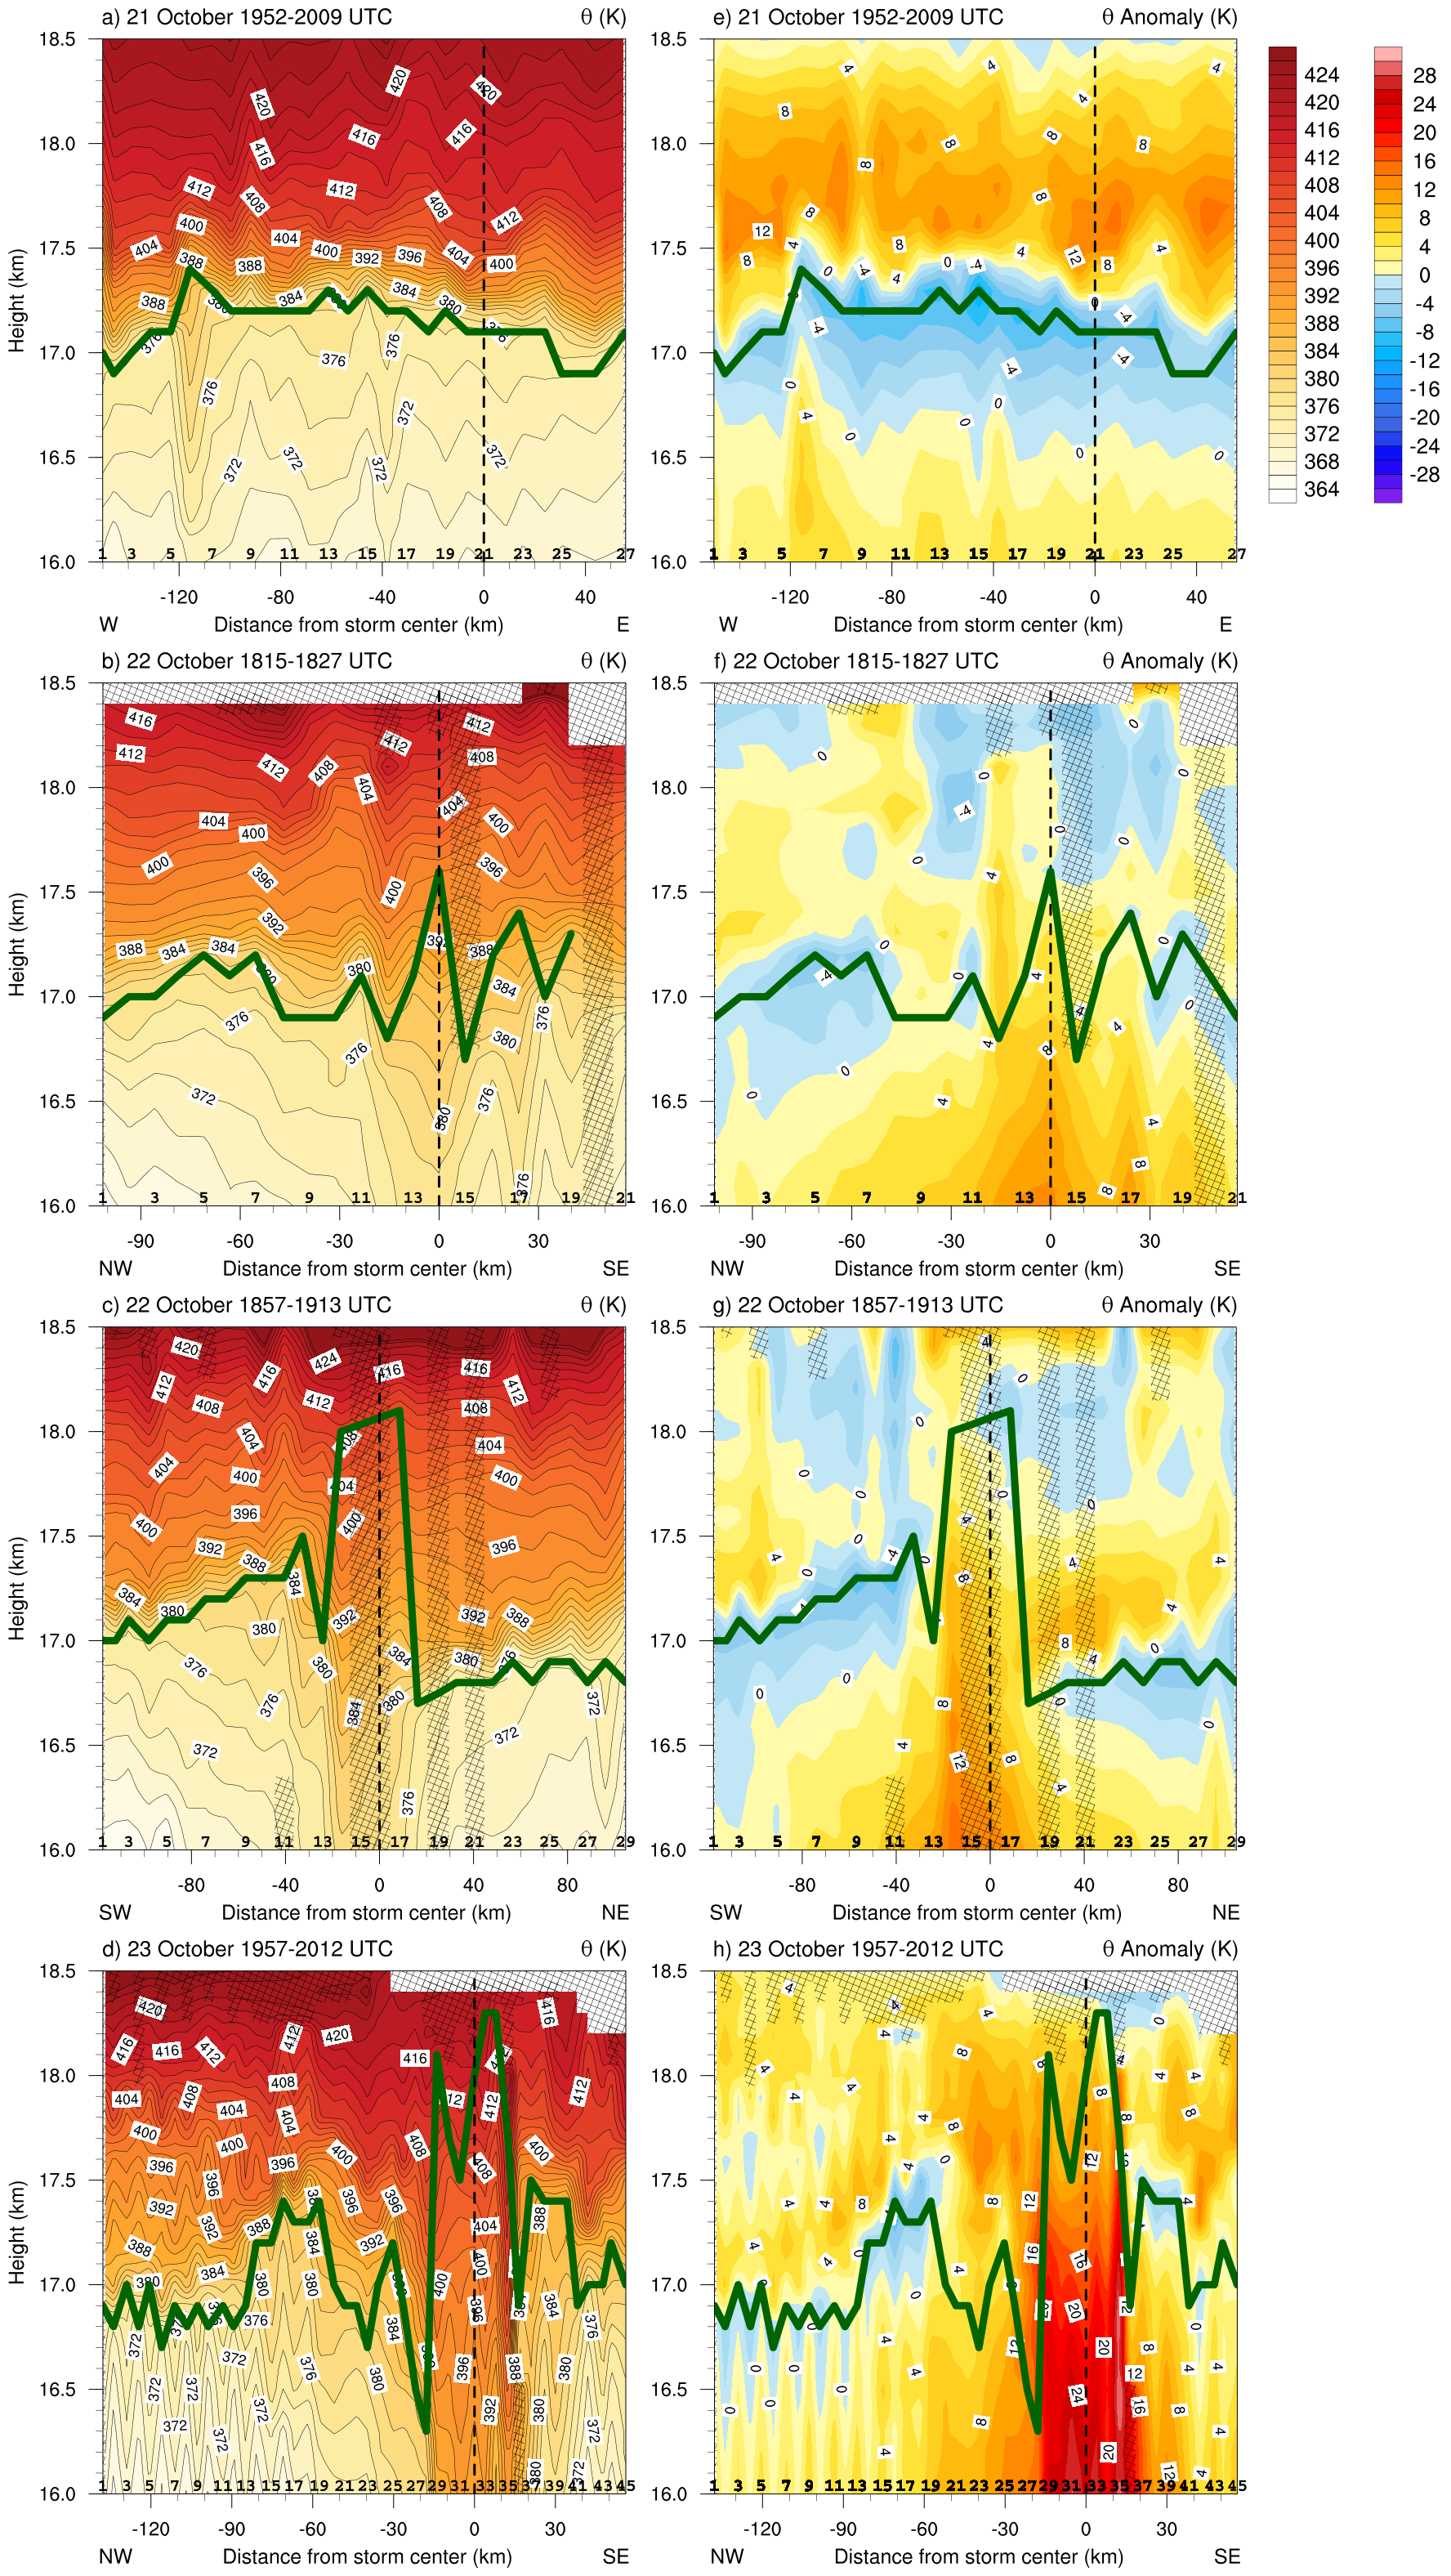
\includegraphics[width=24pc]{figures/fig05_theta+anomalies.png}}
\caption{(left) Vertical cross sections of potential temperature (\textdegree{}C; filled contours) and the cold-point tropopause height (green lines) along the transects shown in Fig. 1 on (a) 21; (b), (c) 22; and (d) 23 Oct 2015. Dropsonde locations, compass directions, and hatching as in Fig. 4. (right) Vertical cross sections of the potential temperature anomaly (\textdegree{}C) on (e) 21; (f),(g) 22; and (h) 23 Oct 2015.}
\label{fig:anomalies}
\end{figure*}

%FIGURE 6%
\begin{figure*}[ht]
\centerline{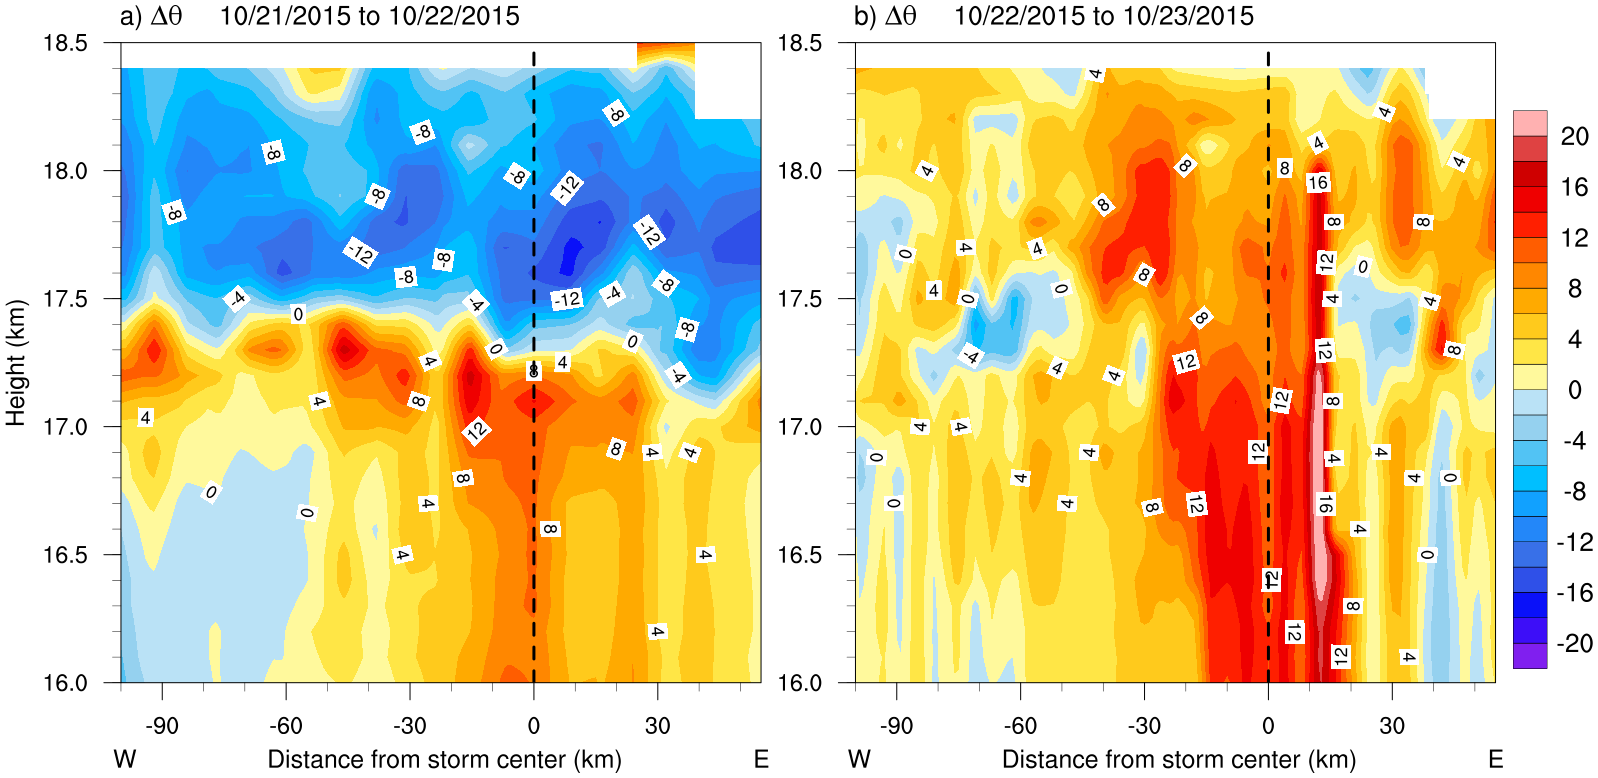
\includegraphics[width=39pc]{figures/fig06_deltatheta.png}}
\caption{Vertical cross sections of the potential temperature change (K day\textsuperscript{-1}) from (a) 21 to 22 Oct and (b) 22 to 23 Oct. These panels extend from the 100-km radius in Patricia’s western semicircle to 55 km in the eastern semicircle. The times separating the transects ($\Delta t$) were 22.45 h (21–22 Oct) and 25.63 h (22–23 Oct). To ease comparison between the two time periods, the potential temperature changes are scaled to 24 h by multiplying by ($24/\Delta t$).}
\label{fig:dtheta}
\end{figure*}

%FIGURE 7%
\begin{figure*}[ht]
\centerline{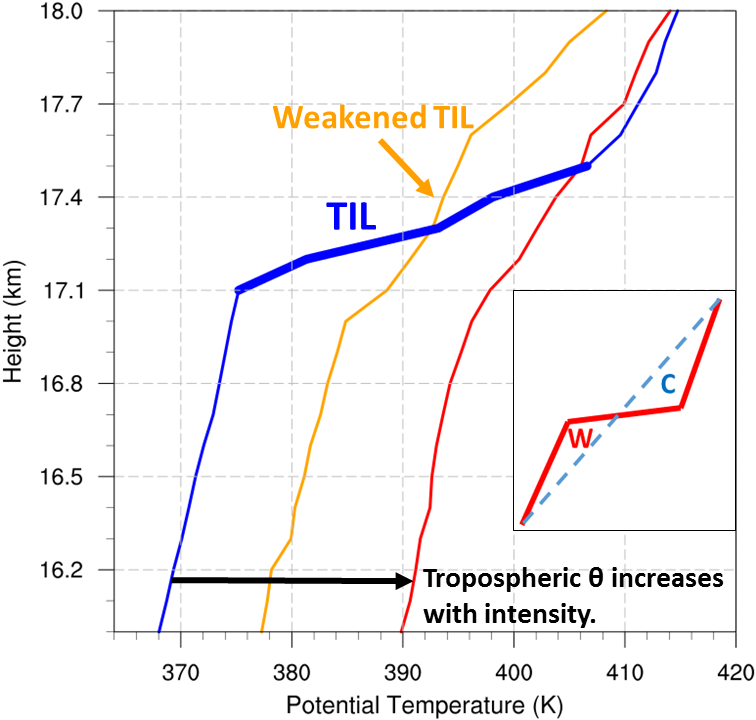
\includegraphics[width=33pc]{figures/fig07_schematic.png}}
\caption{Vertical profiles of potential temperature (K) between 16- and 18-km height for the soundings at Patricia’s storm center on 21 Oct (blue), 22 Oct (orange), and 23 Oct 2015 (red). The bolded segment of the blue line denotes the TIL on 21 Oct. (inset) A simplified schematic of mixing across a strongly stable layer, with the solid red line indicating the initial potential temperature profile and the dashed blue line representing the profile after a period of mixing; ‘‘W’’ and ‘‘C’’ represent regions of warming and cooling, respectively, after mixing.}
\label{fig:schematic}
\end{figure*}

%FIGURE 8%
\begin{figure*}[ht]
\centerline{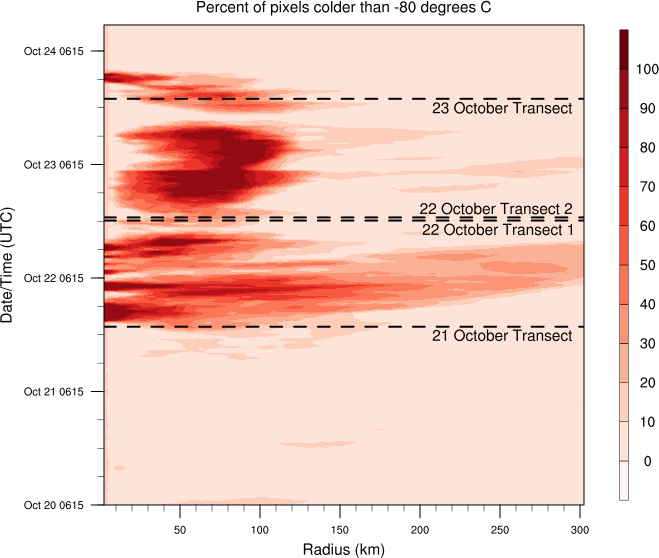
\includegraphics[width=39pc]{figures/fig08_hovmoller_tbpercent.png}}
\caption{Radius–time plot of the percent of infrared brightness temperature pixels colder than -80\textdegree{}C. The plot is constructed by counting the number of pixels colder than -80\textdegree{}C in a 5-km-wide radial bin, dividing by the total number of pixels in that bin, and multiplying by 100. This is performed every 5 km, extending from the storm center out to 300-km radius, for each GOES-13 image collected during Patricia’s lifetime (images are available every 30 min). Dashed black lines mark the times at which the WB-57 aircraft crossed over the storm center.}
\label{fig:hovmoller}
\end{figure*}

%FIGURE 9%
\begin{figure*}[ht]
\centerline{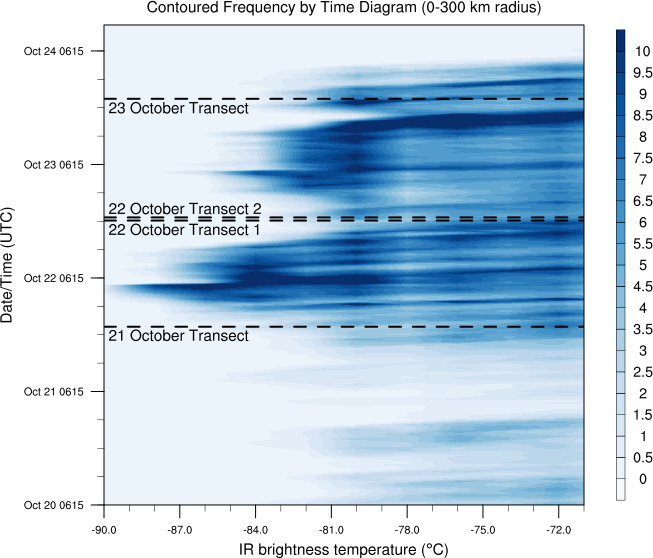
\includegraphics[width=39pc]{figures/fig09_CFTD.png}}
\caption{}
\label{fig:CFTD}
\end{figure*}

%FIGURE 10%
\begin{figure*}[ht]
\centerline{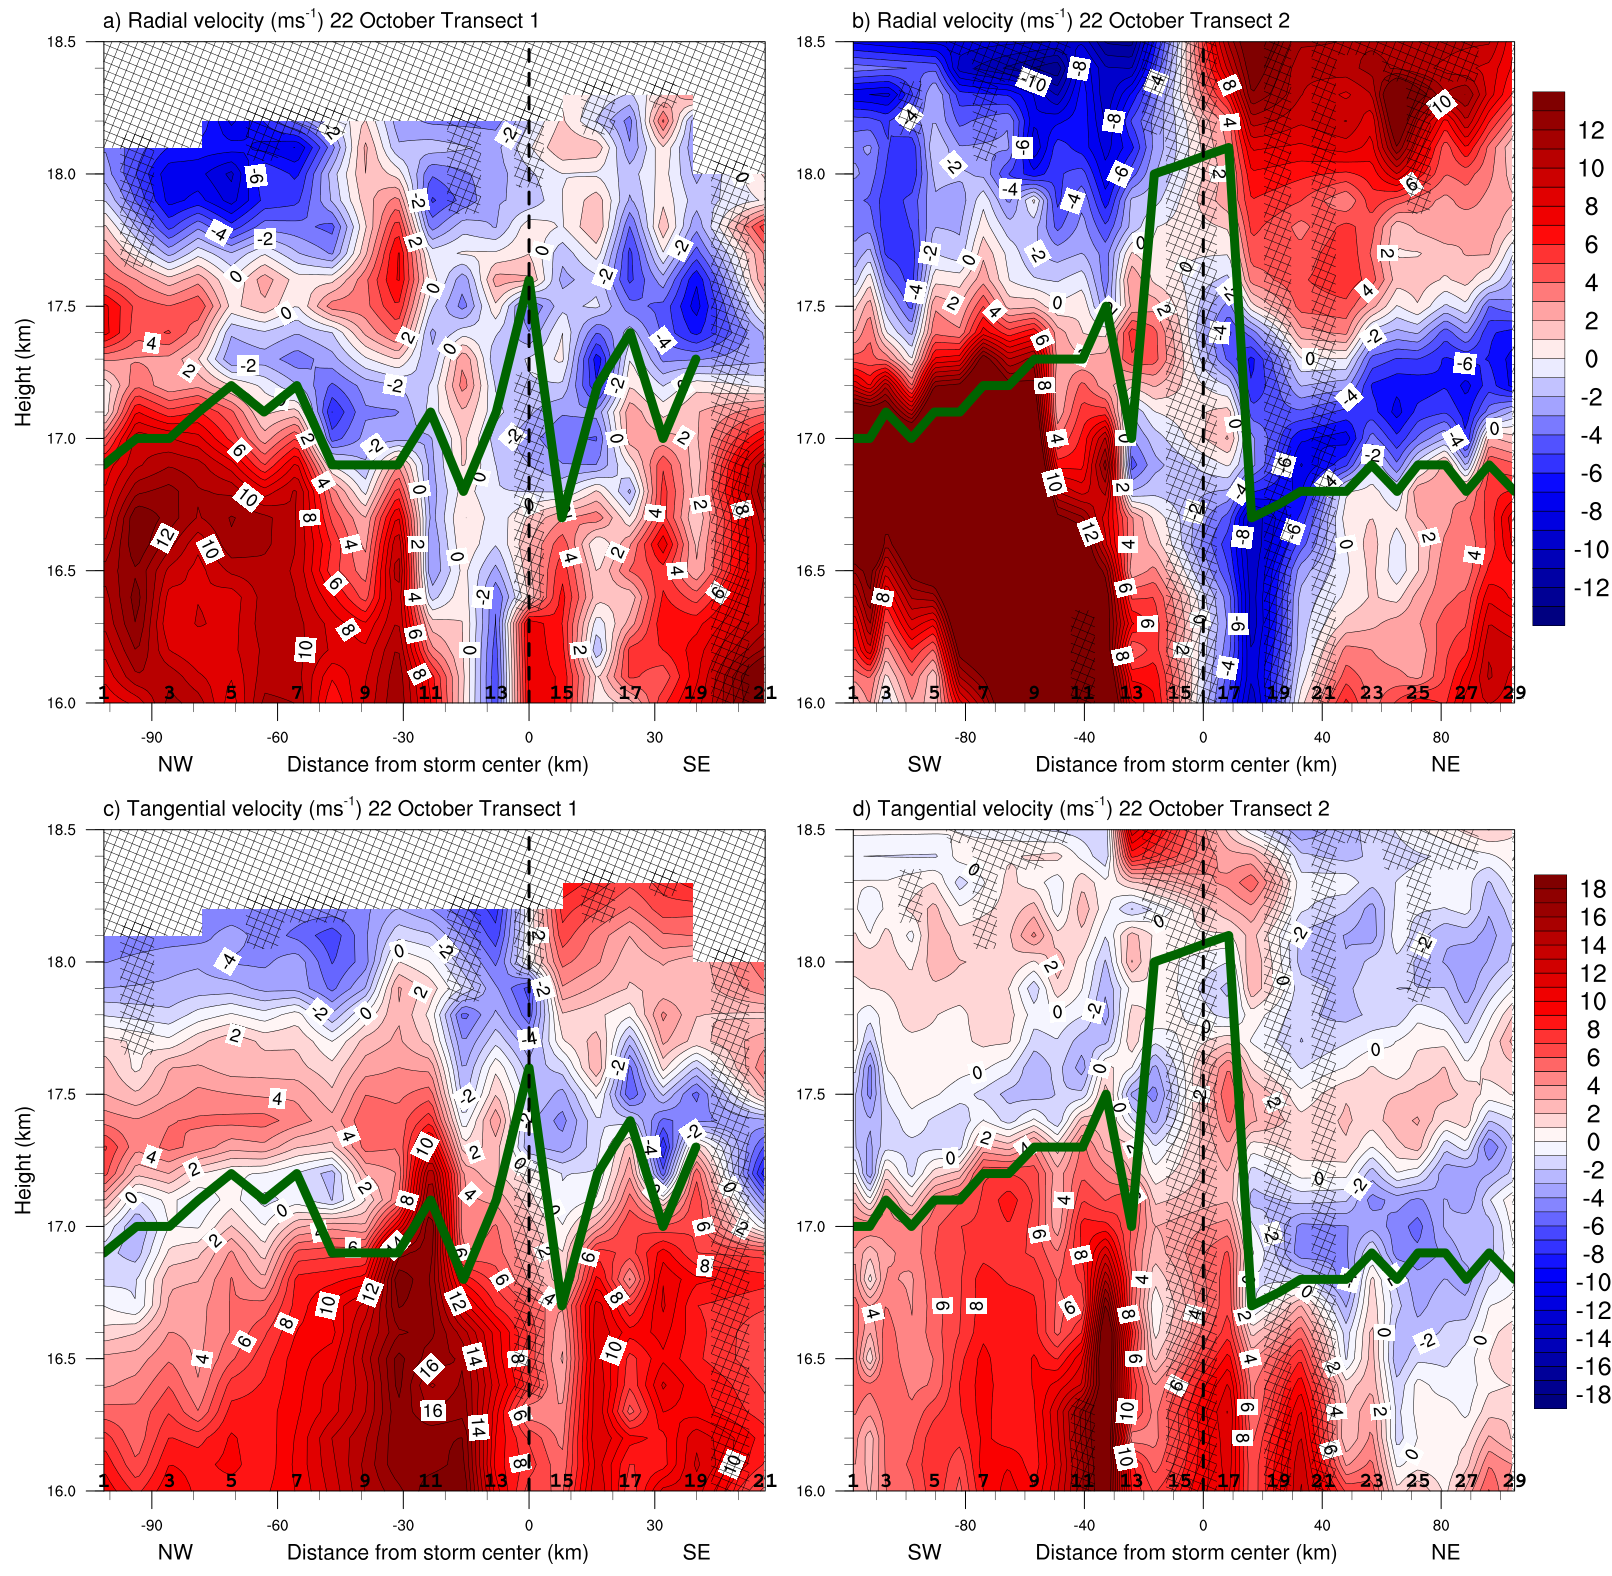
\includegraphics[width=39pc]{figures/fig10_velocities.png}}
\caption{}
\label{fig:velocities}
\end{figure*}
